\documentclass[letterpaper,12pt]{article}
\usepackage[utf8]{inputenc}

\usepackage{rotating}
\usepackage[top=1in, bottom=1in, left=1in, right=1in]{geometry}
\usepackage{graphicx}
\usepackage[numbers,square,sort&compress]{natbib}
\usepackage{setspace}
\usepackage[cdot,mediumqspace,]{SIunits}
\usepackage{hyperref}
\usepackage{mathtools}
\usepackage{url}
\usepackage{authblk}
\usepackage{placeins}
\usepackage{float}

\onehalfspacing
\title{Measuring AU Using Solar Observation}
\author{Anita Bahmanyar \qquad Ayushi Singh \qquad Morten Nyborg Stostad \\Department of Astronomy and Astrophysics, University of Toronto}
\affil{\small {Written by: Anita Bahmanyar}}
\affil{\small {anita.bahmanyar@mail.utoronto.ca}}
\affil{\small {Student Number: 998909098}}
\date{April 2, 2014}

\usepackage{graphicx}

\begin{document}

\maketitle

%Abstract
\begin{abstract}
\label{abstract}
In this lab our goal is to measure the 1 AU in meters by measuring the earth-sun distance with geometry, circular motion and properties of light. We will measure the rotational velocity of the sun using the Doppler shift between each side of the solar limb. We used two methods of finding the covariance and also taking Fourier Transform of the spectrums for this purpose.



\section{Introduction}
\label{sec:introduction}

 
\section{Observation and Data Acquisition}
\label{sec:observationanddataacquisition}
\subsection{Neon and Mercury Lamps}
We used HR1 spectrometer which consists of Toshiba 1 $\times$ 3648 CCD. Size of each pixel is 8 $\mu$ $\times$ 200 $\mu$.  The wavelength range of this spectrometer is 523-573 nm. We used Neon and Mercury lamps to find the wavelength solution for this spectrometer. We set the integration times such that the pixels are not saturated. Therefore, we used 200 ms and 400 ms integration time for neon lamp and 10 ms and 50 ms integration times for the mercury lamp. We also took data of dark counts with the same exposure times for each lamp. 
\subsection{Solar Observing}
We went up to 16th floor of Burton Tower to use the 8-inch refractor telescope for our purpose. We mounted another telescope cap in front of the telescope aperture in order to reduce the amount of light coming into telescope from the Sun so that we do not hurt our eyes. Then we mounted the projection screen as it can be seen in Figure 1 so that we get the Sun on the screen. Next step was to line up the shadow of the finder scope until it became circle as in Figure 2 and then focused the the telescope to get a sharp image(We did this by looking at the sharpness of the sun spots). The next thing we need to consider is the temperature of the spectrometer since the spectral resolution and dispersion of the the spectograph or in general, the wavelength solution changes with temperature and for this mean we placed the spectrometer inside a box to keep the temperature approximately as it was in the astronomy lab, where we collected Neon and Mercury data to solve for the wavelength solution. The box consisted of a resistor that heats up the box. Then we connected the fibre coupler to collimate [....] 

% images a and 2 (flat and centroids)
\begin{figure}[ht]
\centering
\begin{minipage}[b]{0.4\linewidth}
  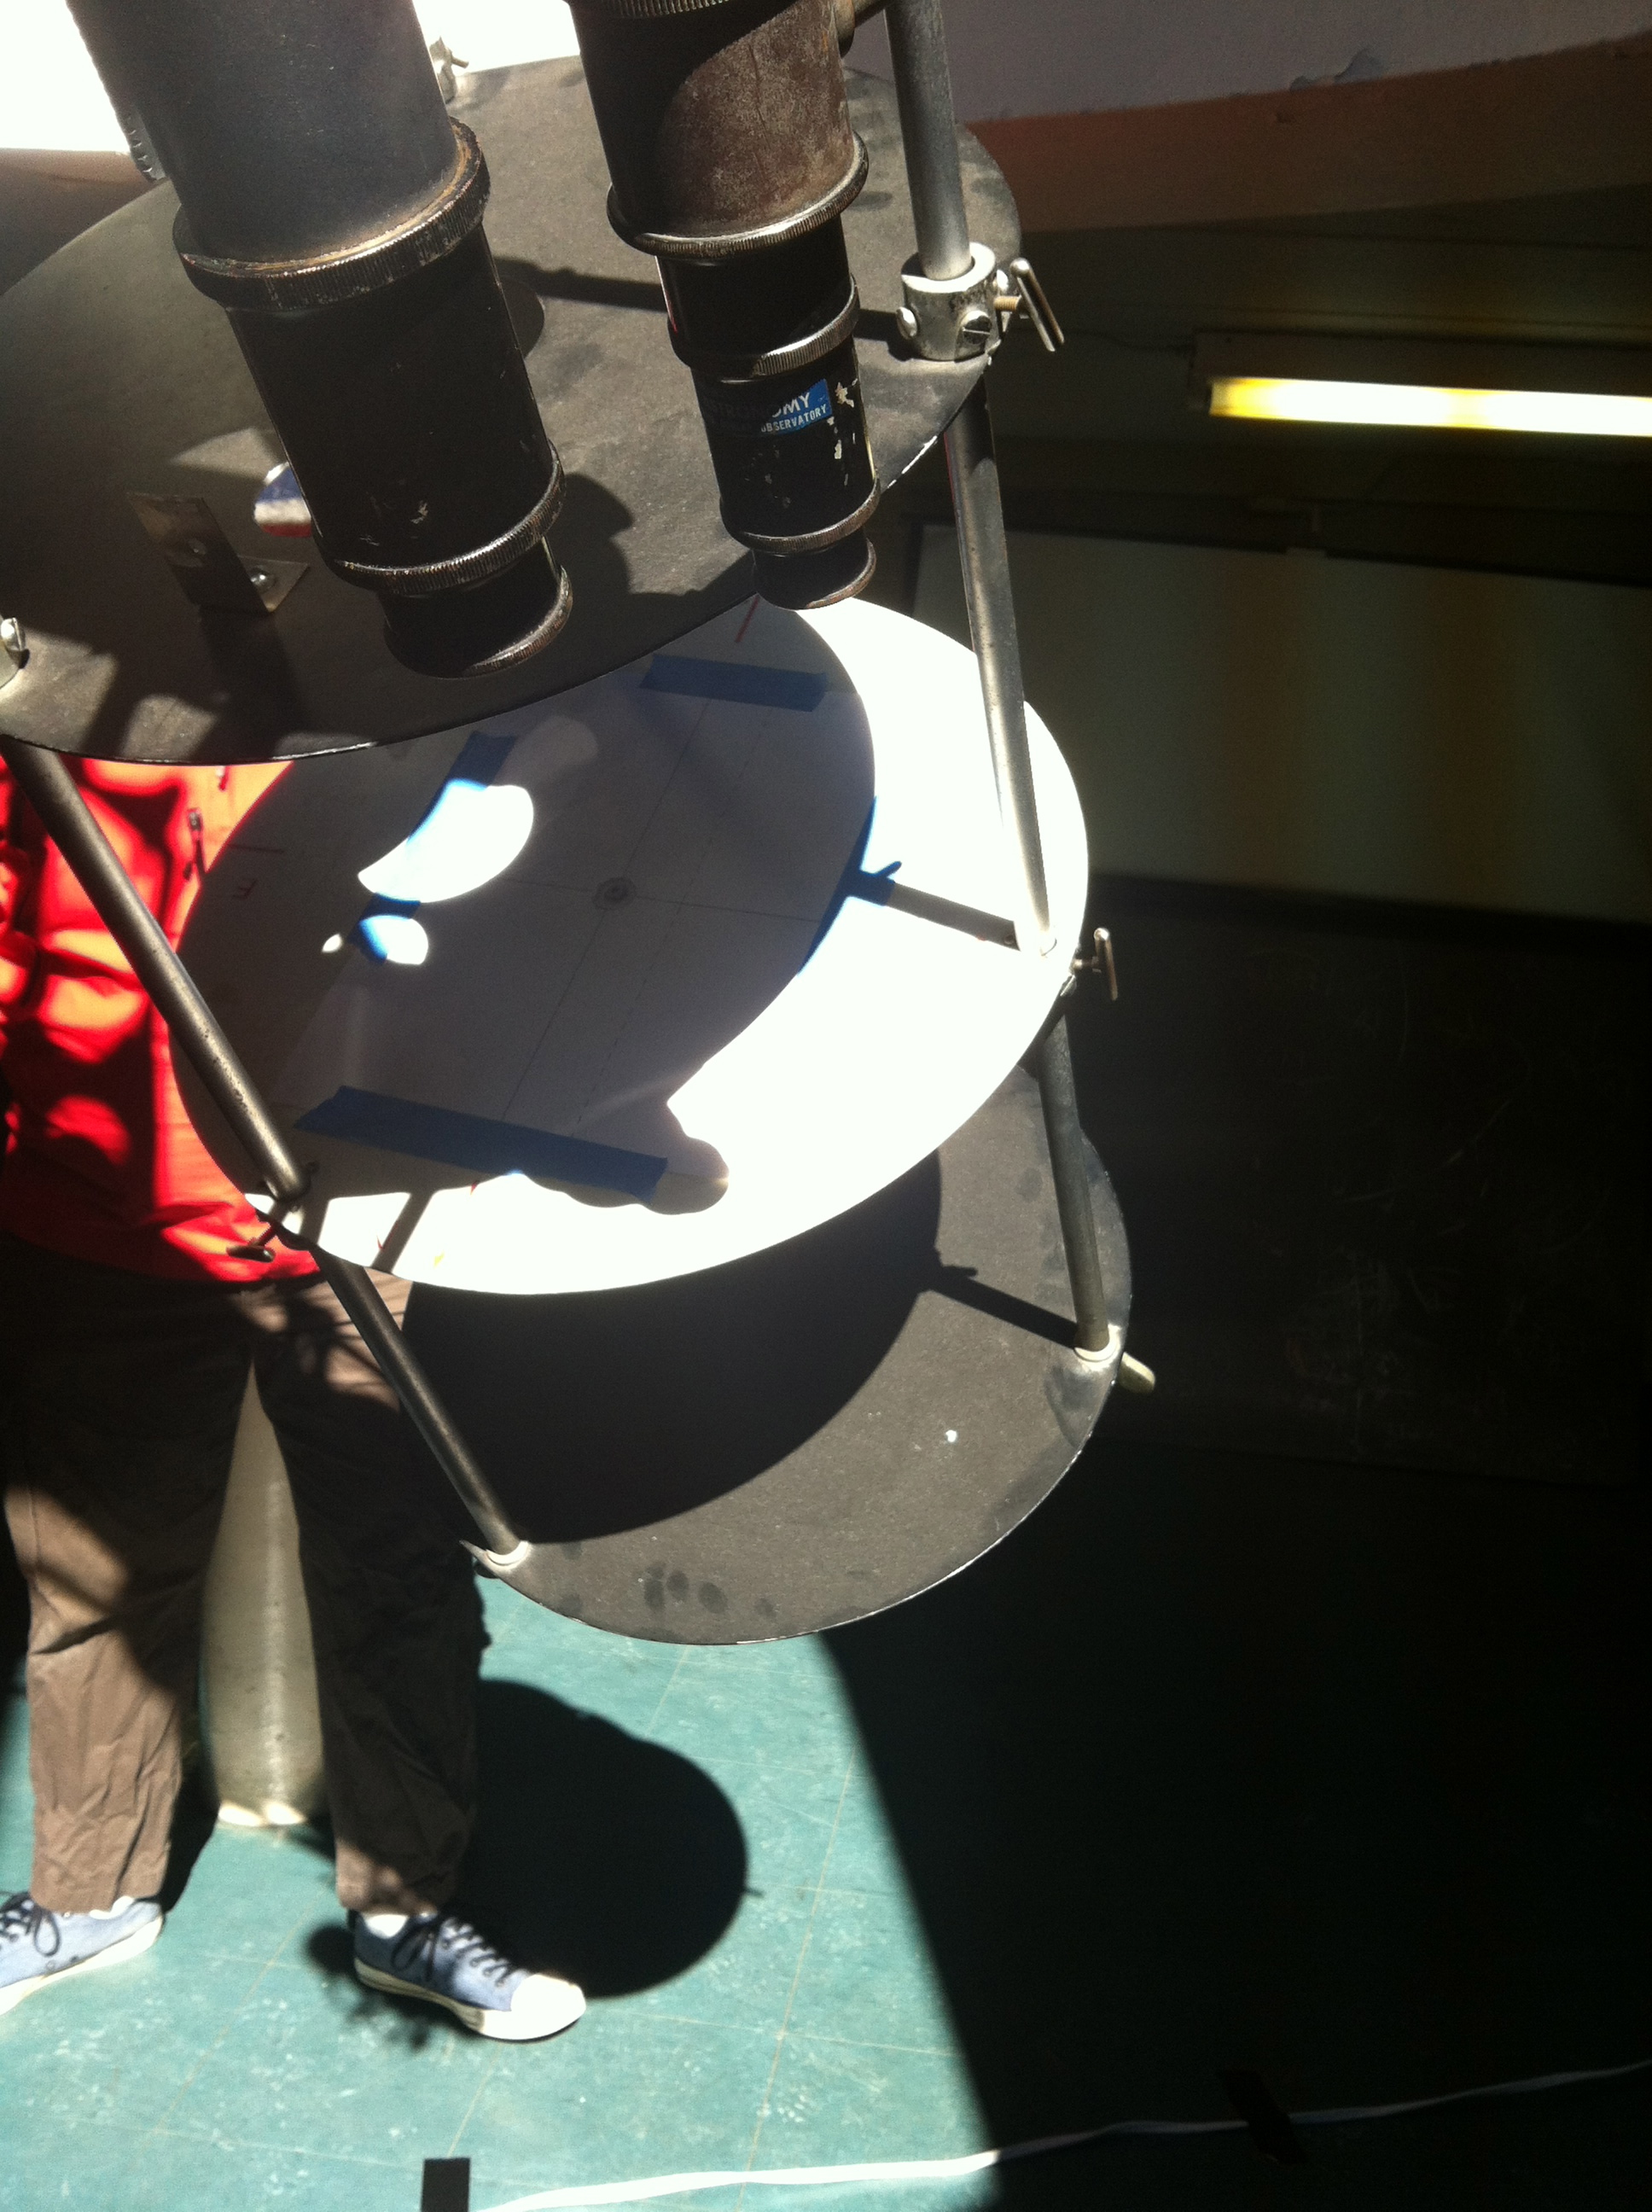
\includegraphics[scale=0.09]{projection.jpg}
  \caption{This figure shows the projection screen mounted on the telescope to get and the image of the Sun on the screen(indirect observing)}
  \label{fig:minipage1}
\end{minipage}
\quad
\begin{minipage}[b]{0.4\linewidth}
  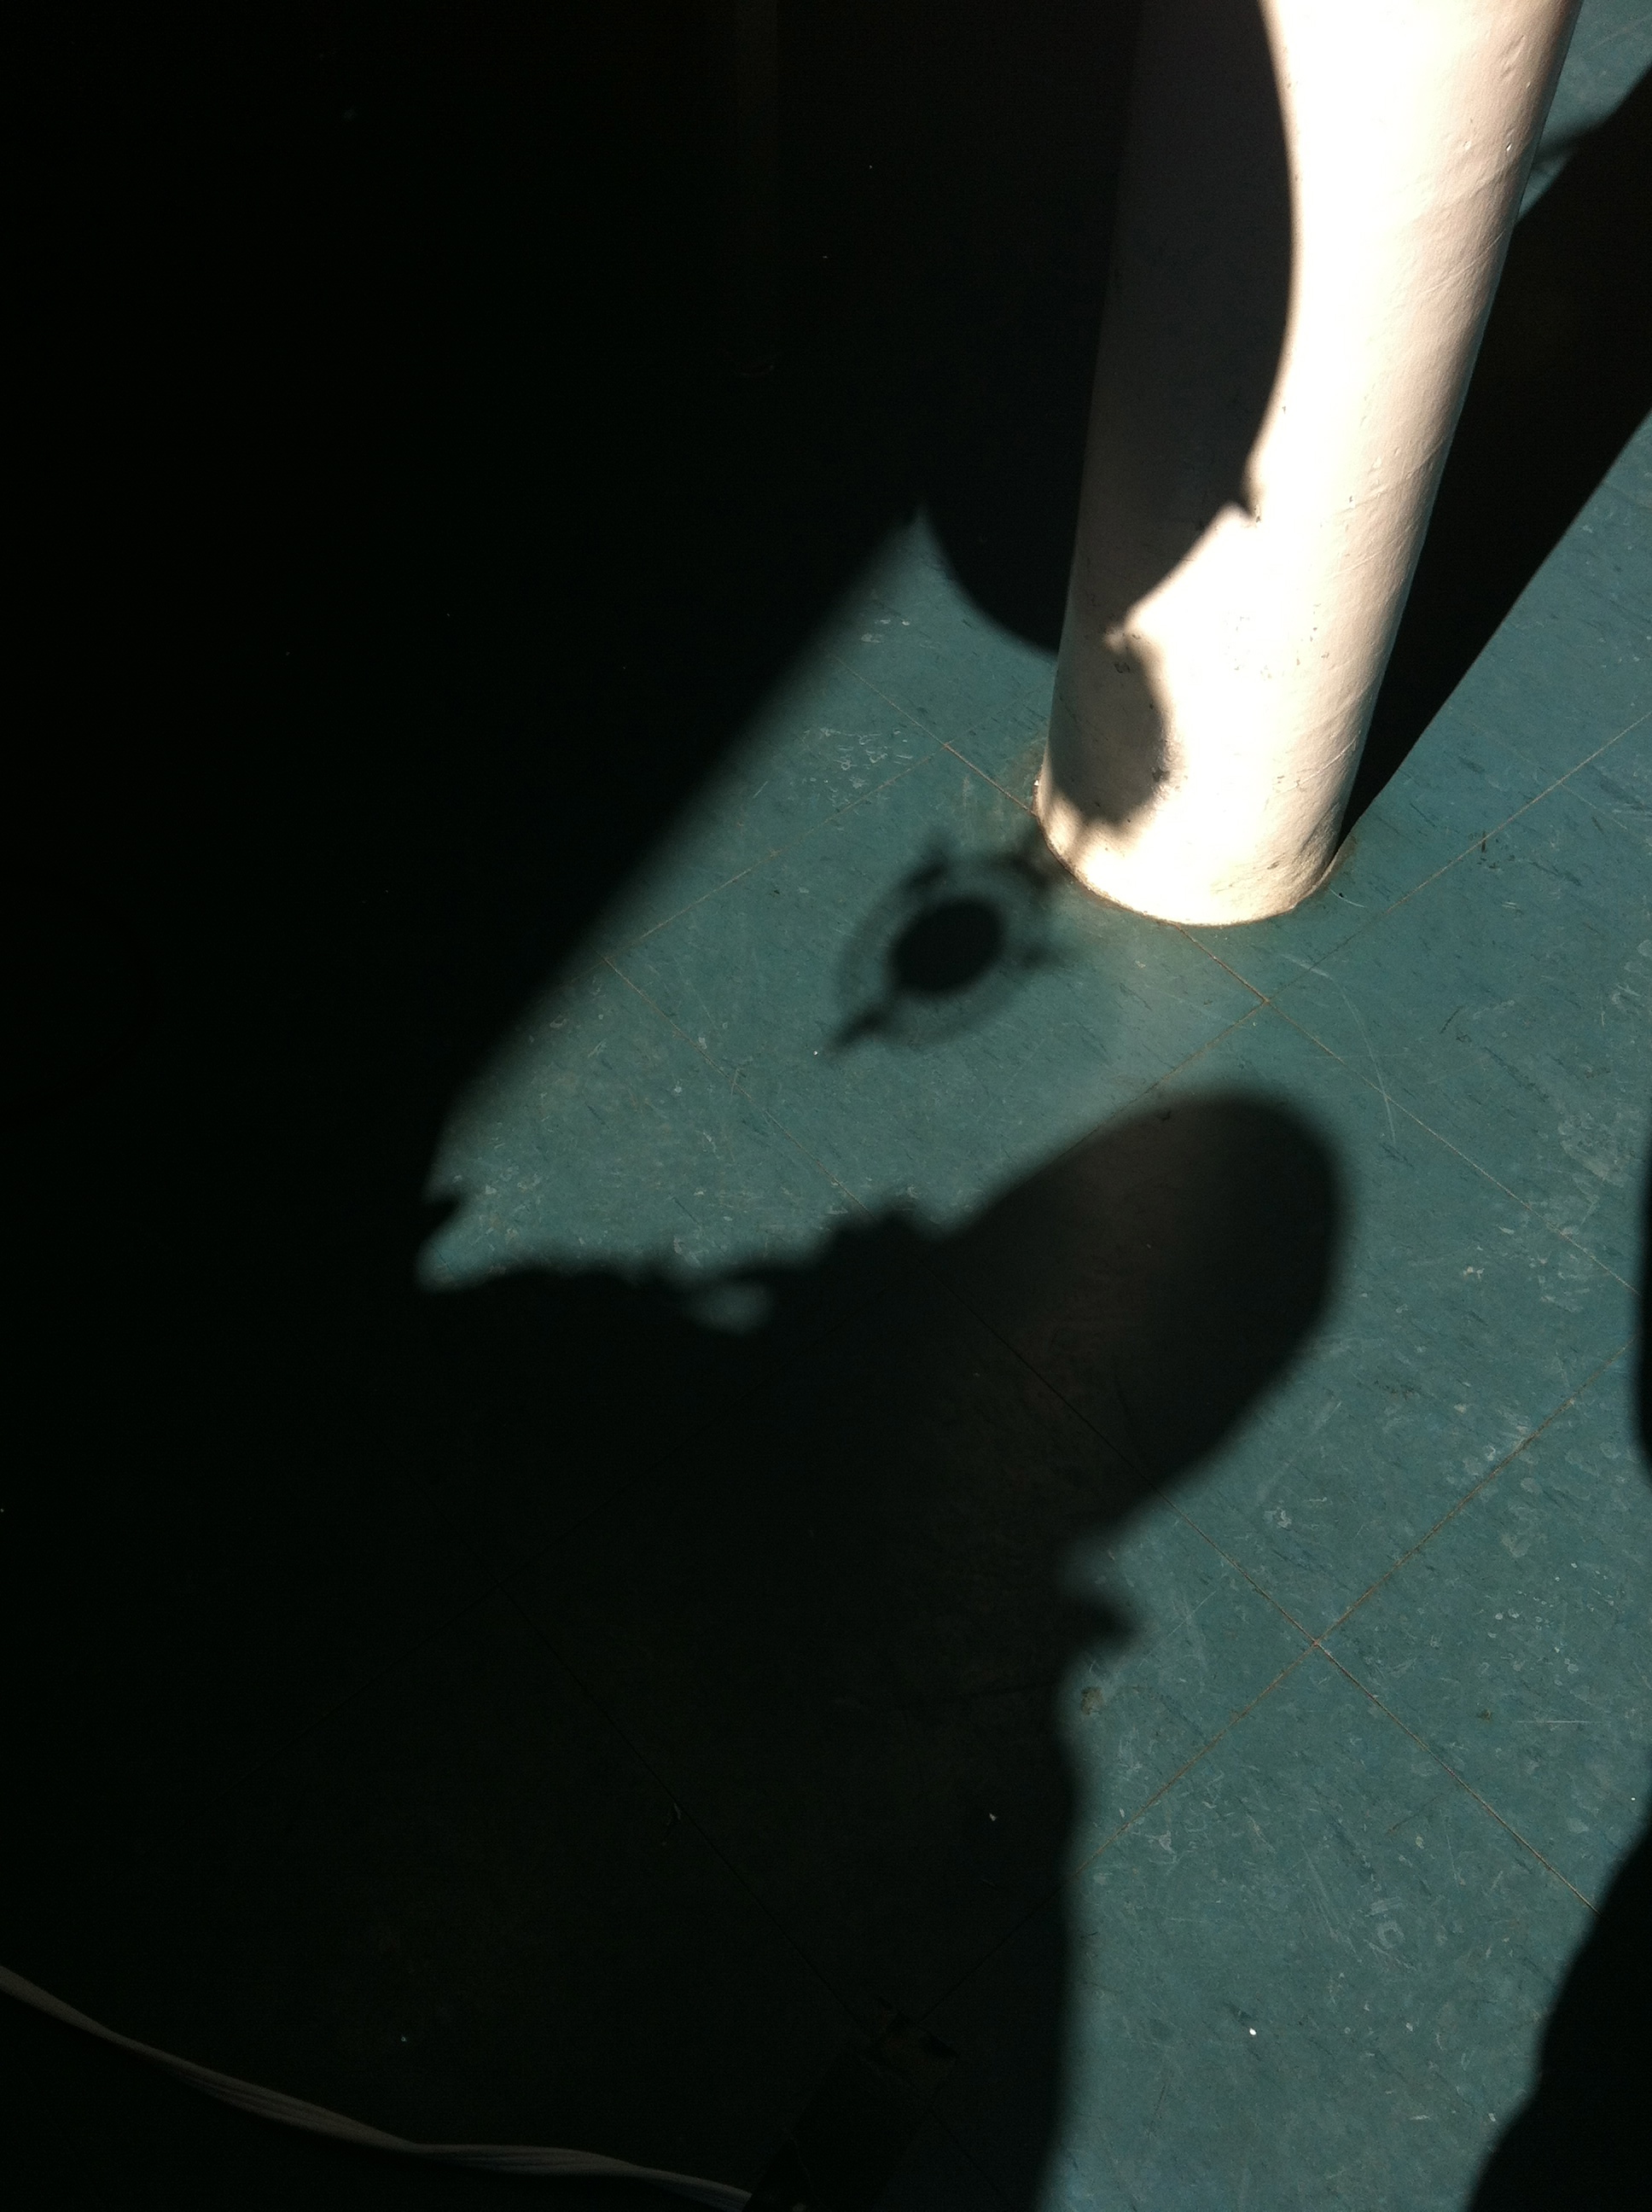
\includegraphics[scale=0.09]{finder-lineup.jpg}
  \caption{This figure shows the shadow of the finder scope as a circle which means it is lined up correctly. We also focused the telescope.}
\label{fig:minipage2}
\end{minipage}
\end{figure}




\section{Analysis}
\label{sec:analysis}
\subsection{Wavelength Solution}
We calibrated the wavelength of the spectrometer since we need to figure out how wavelength is related to the pixel numbers to the wavelength. We used neon and mercury lamps for this purpose. We took 200, 400 and 1000 ms integration times for neon and 10 and 50 ms integration times of data for mercury as well as dark data sets for all of these integration times. We then subtracted dark from the data sets. Figure [....] shows the the intensity vs. pixel number of 10ms mercury and 200ms neon lamp graphs.
We then found the peaks of the graph using centroid method as discussed in Appendix section. Then we compared these peaks with a reference peak wavelength for neon and mercury in the spectrometer wavelength range and plotted the wavelengths vs. pixel numbers in order to find the wavelength solution. We used linear least squares to fit the graph. This was done manually in Python as explained in Appendix, so it means we did not use the built-in package of Python. Fig. [...] shows the wavelength solution, which is $y=0.014 x +524.61$, where $y$ is the wavelength and $x$ is the pixel number. 



\FloatBarrier
\begin{figure}[h!]
\centering
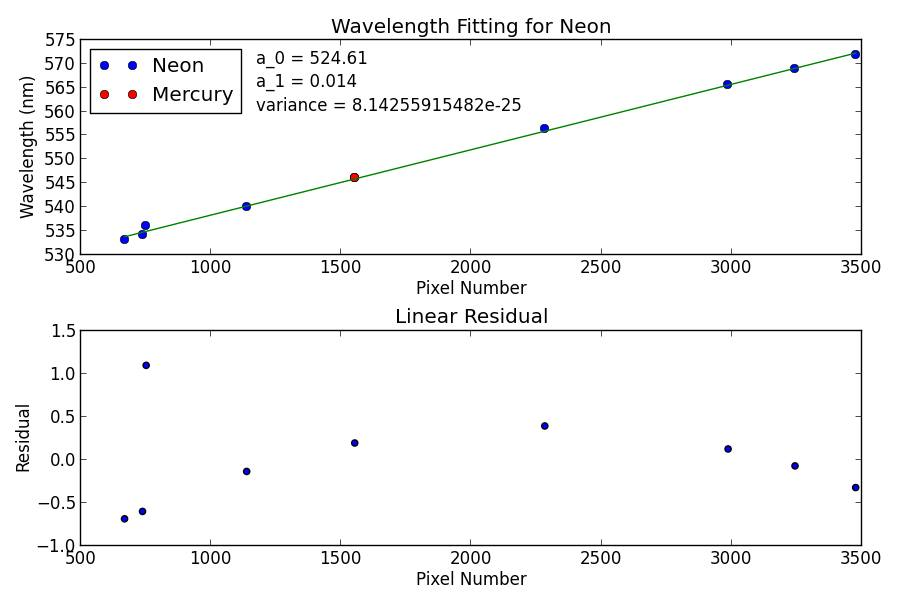
\includegraphics[scale=0.3]{wavelengh_solution.jpg}
\caption{The upper image shows the wavelengths vs. pixel numbers of neon and mercury peaks as compared with their reference spectrum. The wavelength solution is written in the graph. The lower image shows the error in the data and as it is visible it is very small and the variance is also very small that is negligible.}
\end{figure}
\FloatBarrier

Figurea [...] and [...] show the intensity vs. wavelength for neon 200ms and mercury 10ms.

\begin{figure}[ht]
\centering
\begin{minipage}[b]{0.5\linewidth}
  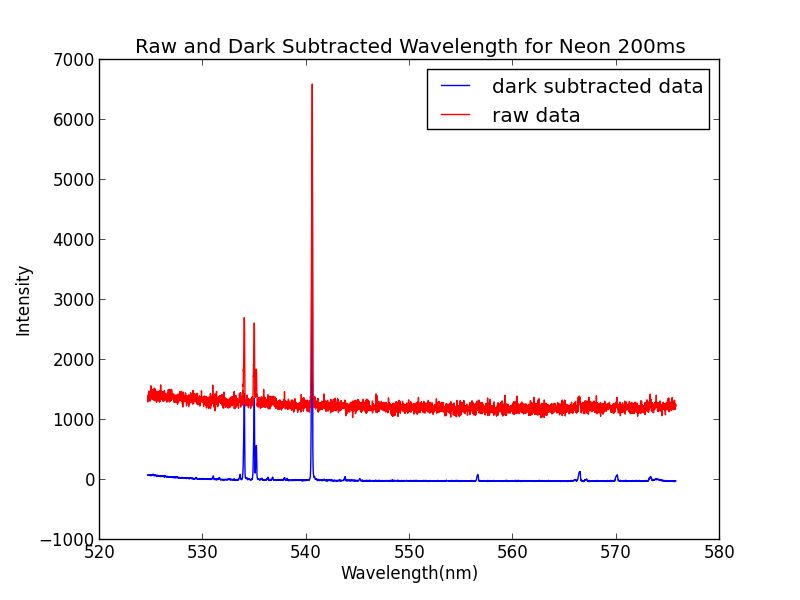
\includegraphics[scale=0.4]{wavelength_neon200ms.png}
  \caption{This figure shows the intensity vs. wavelength of neon 200ms. The raw data is very noisy unlike the mercury raw data.}
  \label{fig:minipage1}
\end{minipage}
\quad
\begin{minipage}[b]{0.4\linewidth}
  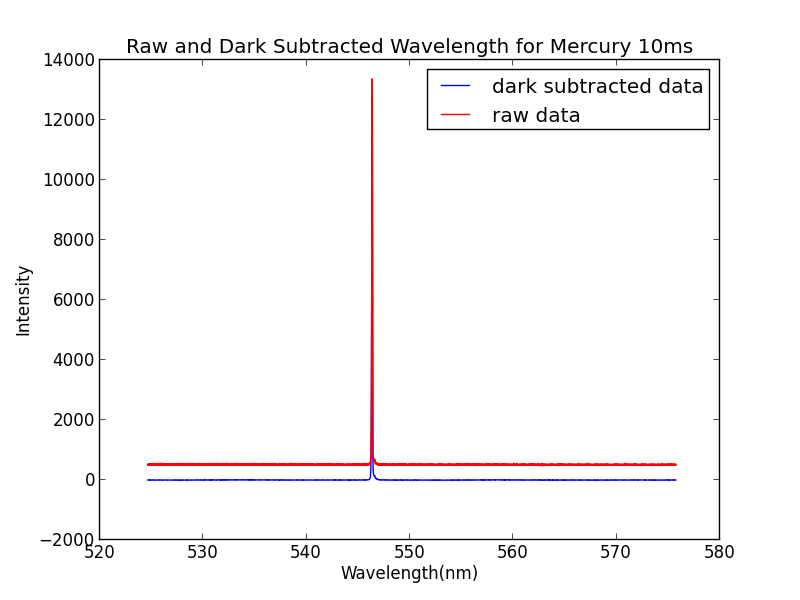
\includegraphics[scale=0.4]{wavelength_merc10ms.png}
  \caption{This figure shows the intensity vs. wavelength of mercury 10ms.}
\label{fig:minipage2}
\end{minipage}
\end{figure}

\subsection{Solar Data}
After finding the wavelength solution of the spectrometer, we should work with solar data. One of the solar data spectrums is plotted vs. wavelength in Fig. [...].



We collected 170ms and 200ms data sets on March 13, 2014 and three sets of data with 125ms integration time on March 18, 2014. We found the mean of each data file and plotted these mean values vs. time. The times where extracted from the file names as it will be discussed in details in Appendix. Then we considered the limb darkening which is given by equation [...]:

\begin{equation}
I=\frac{2}{5}I_{0}(\frac{3}{5}+\sqrt{\frac{(t-t_{0})^2}{\Delta t^2}})
\end{equation}

$I_{0}$ is the intensity of the center value, $\Delta t$ is the difference in the time of the two start and end point data$ and $t_{0}$ is the time of the center data





\section{Discussion}
\label{discussion}


\section{Conclusion}
\label{sec:conclusion}

\section{References}
\label{sec:references}
1-http://www.aseq-instruments.com/HR1.html
2-The lecture slides


\section{Appendix}
\label{sec:appendix}







\end{document}